\documentclass[a4paper,14pt]{extreport}

% =====Задание кодировки=====
\usepackage[utf8]{inputenc}
\usepackage[english,russian]{babel}
% ===========================



% =====Размеры полей=====
\usepackage[left=3cm, right=1.5cm, vmargin=2cm]{geometry}
% =======================



% =====Полуторный интервал=====
\linespread{1.25}
% =============================



% =====Красная строка=====
\usepackage{indentfirst}
\setlength\parindent{1.25cm}
% ========================



% =====Формат заголовков=====
\usepackage{titlesec}

\titleformat
	{\chapter}
	[block]
	{\filcenter\bfseries}
	{\thechapter}
	{1ex}{}
\titlespacing{\chapter}{0pt}{*1}{*1}

\titleformat
	{\section}
	[block]
	{\hspace{\parindent}\bfseries}
	{\thesection}
	{1ex}{}
\titlespacing{\section}{0pt}{*1}{*1}

\titleformat
	{\subsection}
	[block]
	{\hspace{\parindent}\bfseries}
	{\thesubsection}
	{1ex}{}
\titlespacing{\subsection}{0pt}{*1}{*1}

\titleformat
	{\subsubsection}
	[runin]
	{\bfseries}
	{\thesubsubsection}
	{1ex}{}[. ]
\titlespacing{\subsubsection}{1.25cm}{*1}{*1}

\titleformat
	{\paragraph}
	[runin]
	{\bfseries}
	{\theparagraph}
	{1ex}{}[. ]
\titlespacing{\paragraph}{1.25cm}{*1}{*1}

\setcounter{secnumdepth}{3}
% ===========================



% =====Содержание=====
\addto{\captionsrussian}{\renewcommand*{\contentsname}{СОДЕРЖАНИЕ}}
\usepackage{titletoc}
\dottedcontents{chapter}[0em]{\bfseries}{1em}{1ex}
\dottedcontents{section}[2em]{}{2em}{1ex}
\dottedcontents{subsection}[5em]{}{3em}{1ex}
\usepackage[hidelinks]{hyperref}
% ====================



% =====Поиск по тексту=====
\usepackage{cmap}
% =========================



% =====Выравнивание текста=====
\usepackage{ragged2e}
\usepackage{microtype}
\justifying
\sloppy
\tolerance=500
\hyphenpenalty=10000
\emergencystretch=3em
% =============================



% =====Списки====
\renewcommand{\labelitemi}{--}
\renewcommand{\labelitemii}{--}

\renewcommand{\labelenumi}{\asbuk{enumi})}
\renewcommand{\labelenumii}{\arabic{enumii})}

\usepackage{enumitem}
\makeatletter
\AddEnumerateCounter{\asbuk}{\@asbuk}{ю)}
\makeatother
\setlist{nosep,wide}
\setlist[2]{labelindent=2\parindent}
% ===============



% =====Поддержка изображений и таблиц=====
\usepackage[tableposition=top,singlelinecheck=false]{caption}
\usepackage{subcaption}
\usepackage{multirow}
\usepackage{graphicx}
\usepackage{float}
\usepackage{tabularx,ragged2e,booktabs}

\DeclareCaptionLabelFormat{gostfigure}{Рисунок #2}
\DeclareCaptionLabelFormat{gosttable}{Таблица #2}
\DeclareCaptionLabelSeparator{gost}{~---~}
\captionsetup{labelsep=gost}
\captionsetup*[figure]{labelformat=gostfigure,justification=centering}
\captionsetup*[table]{labelformat=gosttable}
\renewcommand{\thesubfigure}{\asbuk{subfigure}}
% ===============================


% =====Листинги=====
\usepackage{minted}
% ==================



\begin{document}
	
\thispagestyle{empty}
\begin{center}

МИНИСТЕРСТВО ВЫСШЕГО ОБРАЗОВАНИЯ И НАУКИ РОССИЙСКОЙ ФЕДЕРАЦИИ
ФЕДЕРАЛЬНОЕ ГОСУДАРСТВЕННОЕ БЮДЖЕТНОЕ
ОБРАЗОВАТЕЛЬНОЕ УЧРЕЖДЕНИЕ
ВЫСШЕГО ОБРАЗОВАНИЯ

«НОВОСИБИРСКИЙ ГОСУДАРСТВЕННЫЙ ТЕХНИЧЕСКИЙ УНИВЕРСИТЕТ»

\noindent\rule{\textwidth}{0.4pt}

Кафедра вычислительной техники

\begin{figure}[H]
	\centering
	
\includegraphics{title/logo.jpeg}
\end{figure}

Лабораторная работа №3

По дисциплине: «Программное обеспечение информационных систем»

По теме: «Приложение ASP.NET Core для работы с базой данных PostgreSQL»

\end{center}

\noindent\begin{tabular}{p{0.5\textwidth}p{0.5\textwidth}}
	Выполнили: & Проверил: \\
	Студенты гр. <<АВТ-818>>, <<АВТФ>> & << должность >>\\
	<<Жигулин И. О.>> & <<Бычков М. И.>> \\
	<<Сороковикова Е. В.>> & \\
	<<\rule{1.5em}{0.4pt}>> \rule{5em}{0.4pt} 20\rule{1.5em}{0.4pt}г. & <<\rule{1.5em}{0.4pt}>> \rule{5em}{0.4pt} 20\rule{1.5em}{0.4pt}г.\\
	\rule{7.5em}{0.4pt} & \rule{7.5em}{0.4pt} \\
	\hspace{1.5em}(подпись) & \hspace{1.5em}(подпись)
\end{tabular}


\begin{center}

\vspace{2.3cm}

Новосибирск

2021
\end{center}


\tableofcontents

\chapter{ВВЕДЕНИЕ}

\section{Цель}
Получить практические навыки по созданию макета сайта с помощью эталонных страниц.

\section{Вариант}
Пятый вариант предусматривает создание страницы со ссылками на статьи.

\section{Задание}

\begin{itemize}
	\item Создать пустой проект.
	\item Добавить в созданный проект две мастер-страницы с именами по умолчанию.
	\item Добавить в проект представление с главной страницей. При добавлении осуществить выбор нужной мастер-страницы.
\end{itemize}

\chapter{ОСНОВНАЯ ЧАСТЬ}

\section{Описание работы мастер-страниц}
Когда у нас в проекте много представлений, и все они содержат какие-то общие элементы, то вместо того, чтобы пописывать все эти элементы в каждом представлении, гораздо удобнее задать один общий шаблон. В этом случае при изменении каких-то общих элементов будет достаточно изменить один раз в общем шаблоне, не изменяя всех остальных представлений. В ASP.NET Core MVC таким шаблоном являются мастер-страницы.

Мастер-страницы применяются для создания единообразного, унифицированного вида сайта. По сути мастер-страницы - это те же самые представления, которые могут включать в себя другие представления. Например, можно определить на мастер-странице общие для всех остальных представлений меню, а также подключить общие стили и скрипты. В итоге нам не придется на каждом отдельном представлении прописывать путь к файлам стилей, а потом при необходимости его изменять. А специальные теги позволяют вставлять в определенное место на мастер-страницах другие представления.

По умолчанию при создании нового проекта ASP.NET MVC Core в проект уже добавляется мастер-страница под названием \_Layout.chtml, которую можно найти в каталоге Views/Shared.

Код мастер-страницы напоминает полноценную WEB-страницу: здесь присутствуют основные теги <html>, <head>, <body> и так далее. И также здесь могут использоваться конструкции Razor. Фактически это то же самое представление. Главное же отличие от обычных представлений состоит в использовании метода @RenderBody(), который является плейсхолдером и на место которого потом будут подставляться другие представления, использующие данную мастер-страницу. В итоге появляется возможность легко установить для всех представлений WEB-приложения единообразный стиль оформления.

По умолчанию представления уже подключают мастер-страницу за счет файла \_ViewStart.cshtml. Этот файл можно найти в проекте в папке Views. Код этого файла добавляется в самое начало кода преставлений при их запуске. При этом файлы представлений, к которым применяется \_ViewStart.cshtml, должны находиться с этим файлов в одном каталоге.

В каждом представлении через синтаксис Razor доступно свойство Layout, которое хранит ссылку на мастер-страницу. Здесь в качестве мастер страницы устанавливается файл \_Layout.cshtml. При этом расширение можно не использовать.

Когда будет происходить рендеринг представления, то система будет искать мастер страницу \_Layout по следующим путям:

\begin{itemize}
	\item /Views/[Название\_контроллера]/\_Layout.cshtml
	\item /Views/Shared/\_Layout.cshtml
\end{itemize}

Если в обеих папках: и в /Views/[Название\_контроллера], и в /Views/Shared/ имеется файл с одинаковым именем, например, \_Layout.cshtml, то к представлению применяется файл, который находится с ним в одной папке как более приоритетный. То есть таким образом имеется возможность определить для представлений каждого отдельного контроллера или представлений, которые находятся в одной папке, свою отдельную мастер-страницу.

Код из \_ViewStart.cshtml выполняется до любого кода в представлении. И чтобы переопределить мастер-страницу, в представлении достаточно установить свойство Layout. Мы можем вообще не использовать мастер-страницу, тогда нам надо присвоить значение null, Либо можно использовать какую-нибудь уже имеющуюся мастер-страницу, указав к ней полный путь.

Кроме метода RenderBody(), который вставляет основное содержимое представлений, мастер-страниц может также использовать специальный метод RenderSection() для вставки секций. Мастер-страница может иметь несколько секций, куда представления могут поместить свое содержимое.

\section{Создание общей мастер-страницы}
Создадим общую мастер-страницу для всех представлений. Для этого откроем файл Views/\_ViewStart.cshtml и запишем в него следующий код:

\begin{minted}{html}
@{
  Layout = "_Layout";
}
\end{minted}


Затем создадим файл Views/Shares/\_Layout.cshtml, который будет содержать код общей мастер-страницы:

\begin{minted}{HTML}
<!DOCTYPE html>
<html lang="en">
<head>
  <meta charset="UTF-8">
  <meta http-equiv="X-UA-Compatible" content="IE=edge">
  <meta name="viewport"
        content="width=device-width, initial-scale=1.0">
  <title>ПОИС</title>
</head>
<body>
  <header>
    <nav>
      <a href="~/Home/Index">Главная</a>
      <a href="~/Laba1/Index">Лаба 1</a>
      <a href="~/Laba2/Index">Лаба 2</a>
      <a href="~/Laba3/Index">Лаба 3</a>
      <a href="~/Laba4/Index">Лаба 4</a>
      <a href="~/RGR/Index">РГР</a>
    </nav>
  </header>

  <main>
    @RenderBody()
  </main>

  <footer>
    <small>
      Жигулин И. О., Сороковикова Е. В., АВТ-818, 2021 г.
    </small>
  </footer>
</body>
</html>
\end{minted}

В созданной мастер странице можно выделить верхнюю часть --- header и нижнюю --- footer. Верхняя содержит меню сайта со ссылками на главную страницу и на страницы соответствующих лабораторных работ. Нижняя --- информацию об авторах.

\section{Создание специфичной мастер-страницы и статей}
Теперь создадим специальную мастер страницу для данной лабораторной работы, которая будет содержать ссылки на статьи и ссылку для возврата назад. Для этого создадим файл /Views/Laba2/\_Layout.cshtml и заполним его так:

\begin{minted}{HTML}
<ul>
  <li><a href="~/Laba2/Index">Превью</a></li>
  <li><a href="~/Laba2/About">Об авторах</a></li>
  <li><a href="~/Laba2/Test">Тест</a></li>
  <li><a href="~/Home/Index">Назад</a></li>
</ul>

@RenderBody()
\end{minted}

Теперь создадим небольшие файлы, которые содержат код статей: Views/Laba2/Index.cshtml, Views/Laba2/About.cshtml, Views/Laba2/Test.cshtml. Они не содержат ничего, кроме HTML-абзацев, которые позволяют идентифицировать эти страницы.

\section{Создание контроллера}
Создадим контроллер, который будет обрабатывать полученные запросы к статьям. Это сделаем с помощью файла /Controllers/Laba2Controller.cshtml:

\begin{minted}{csharp}
namespace Labs.Controllers
{
  public class Laba2 : Controller
  {        
    public IActionResult Index()
    {
      return View();
    }
		
    public IActionResult About()
    {
      return View();
    }
		
    public IActionResult Test()
    {
      return View();
    }
  }
}
\end{minted}

Разработанный контроллер содержит три метода, каждый из которых возвращает свое представление. Эти представления содержат только текст. Список со ссылками на страницы заданы в специфичной для данной лабораторной мастер-странице.


\chapter{ЗАКЛЮЧЕНИЕ}

\section{Демонстрация работы}


\begin{figure}[H]
	\centering
	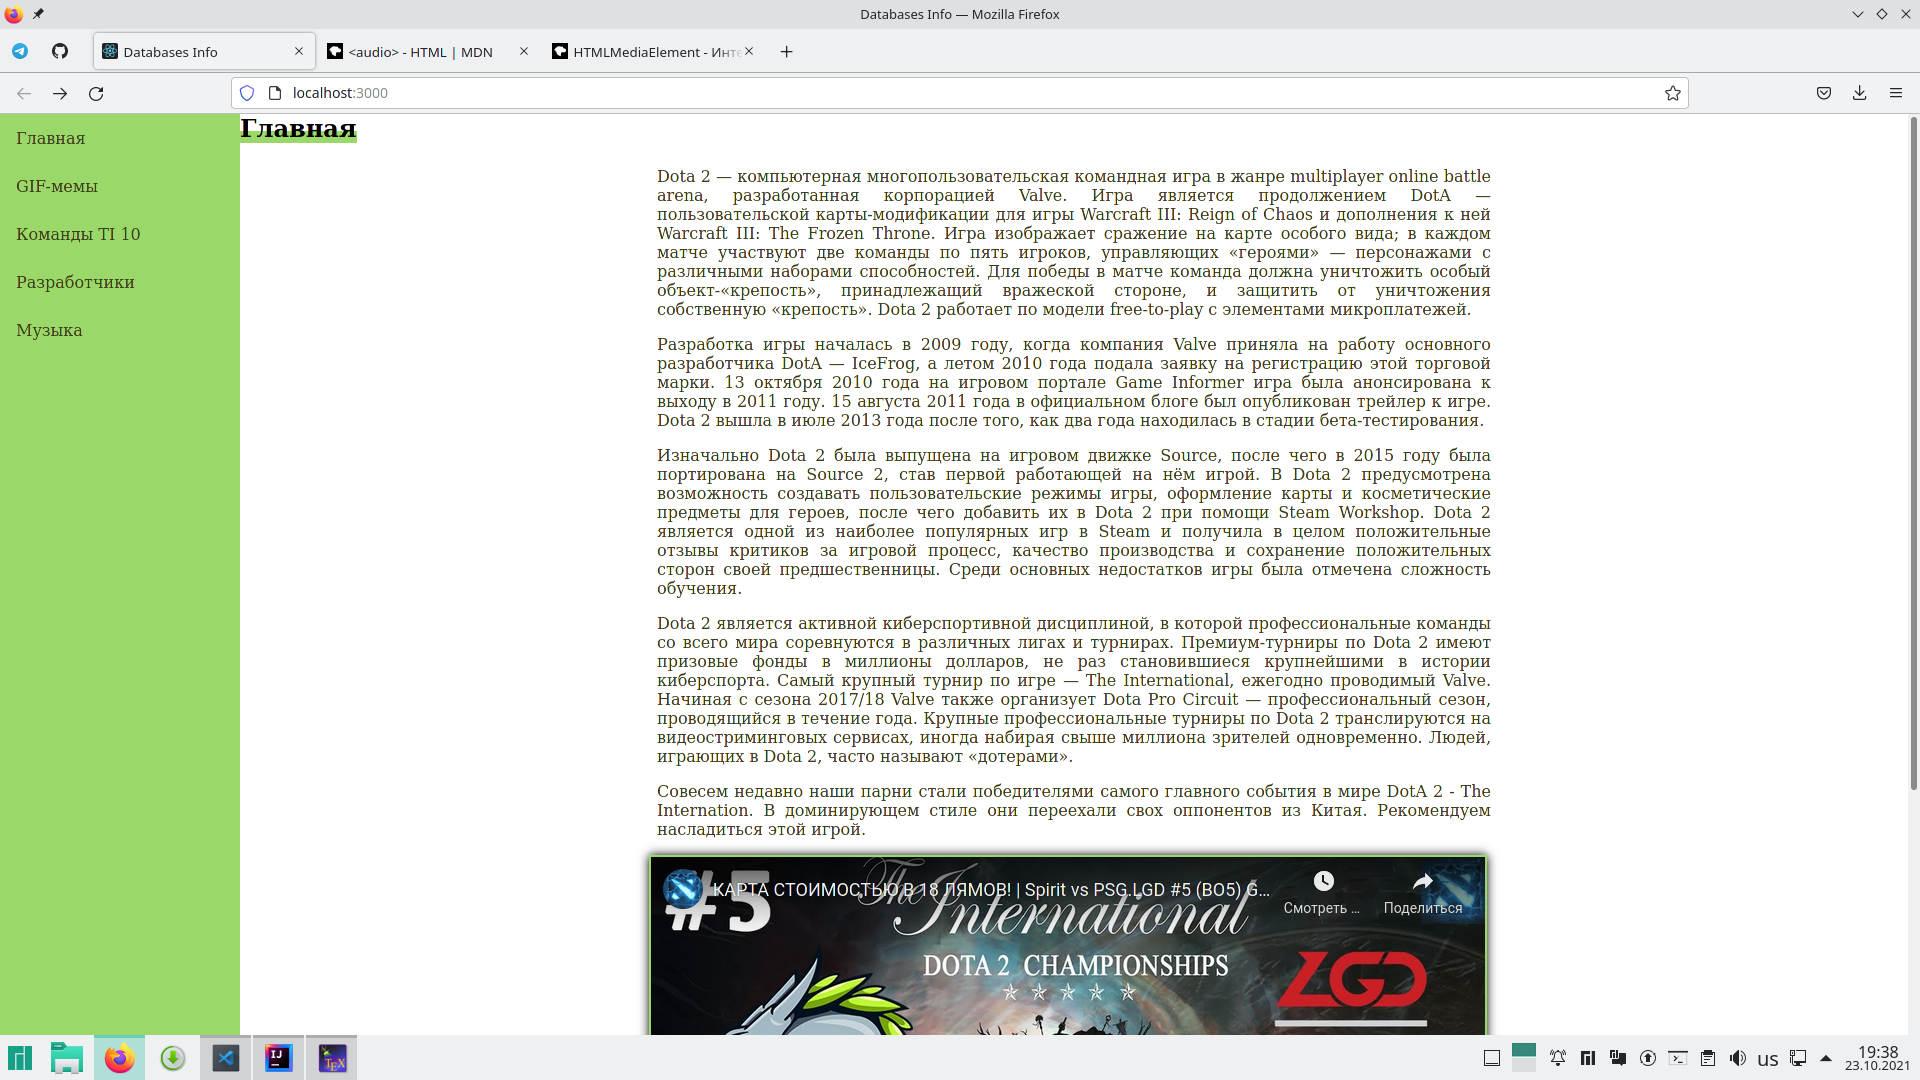
\includegraphics{01}
	\caption{Общая мастер-страница}
\end{figure}

\begin{figure}[H]
	\centering
	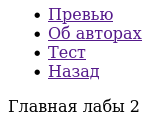
\includegraphics{02}
	\caption{Первая статья специфичной мастер-страницы}
\end{figure}

\begin{figure}[H]
	\centering
	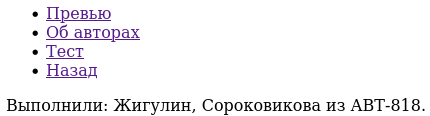
\includegraphics{03}
	\caption{Вторая статья специфичной мастер-страницы}
\end{figure}
\begin{figure}[H]
	\centering
	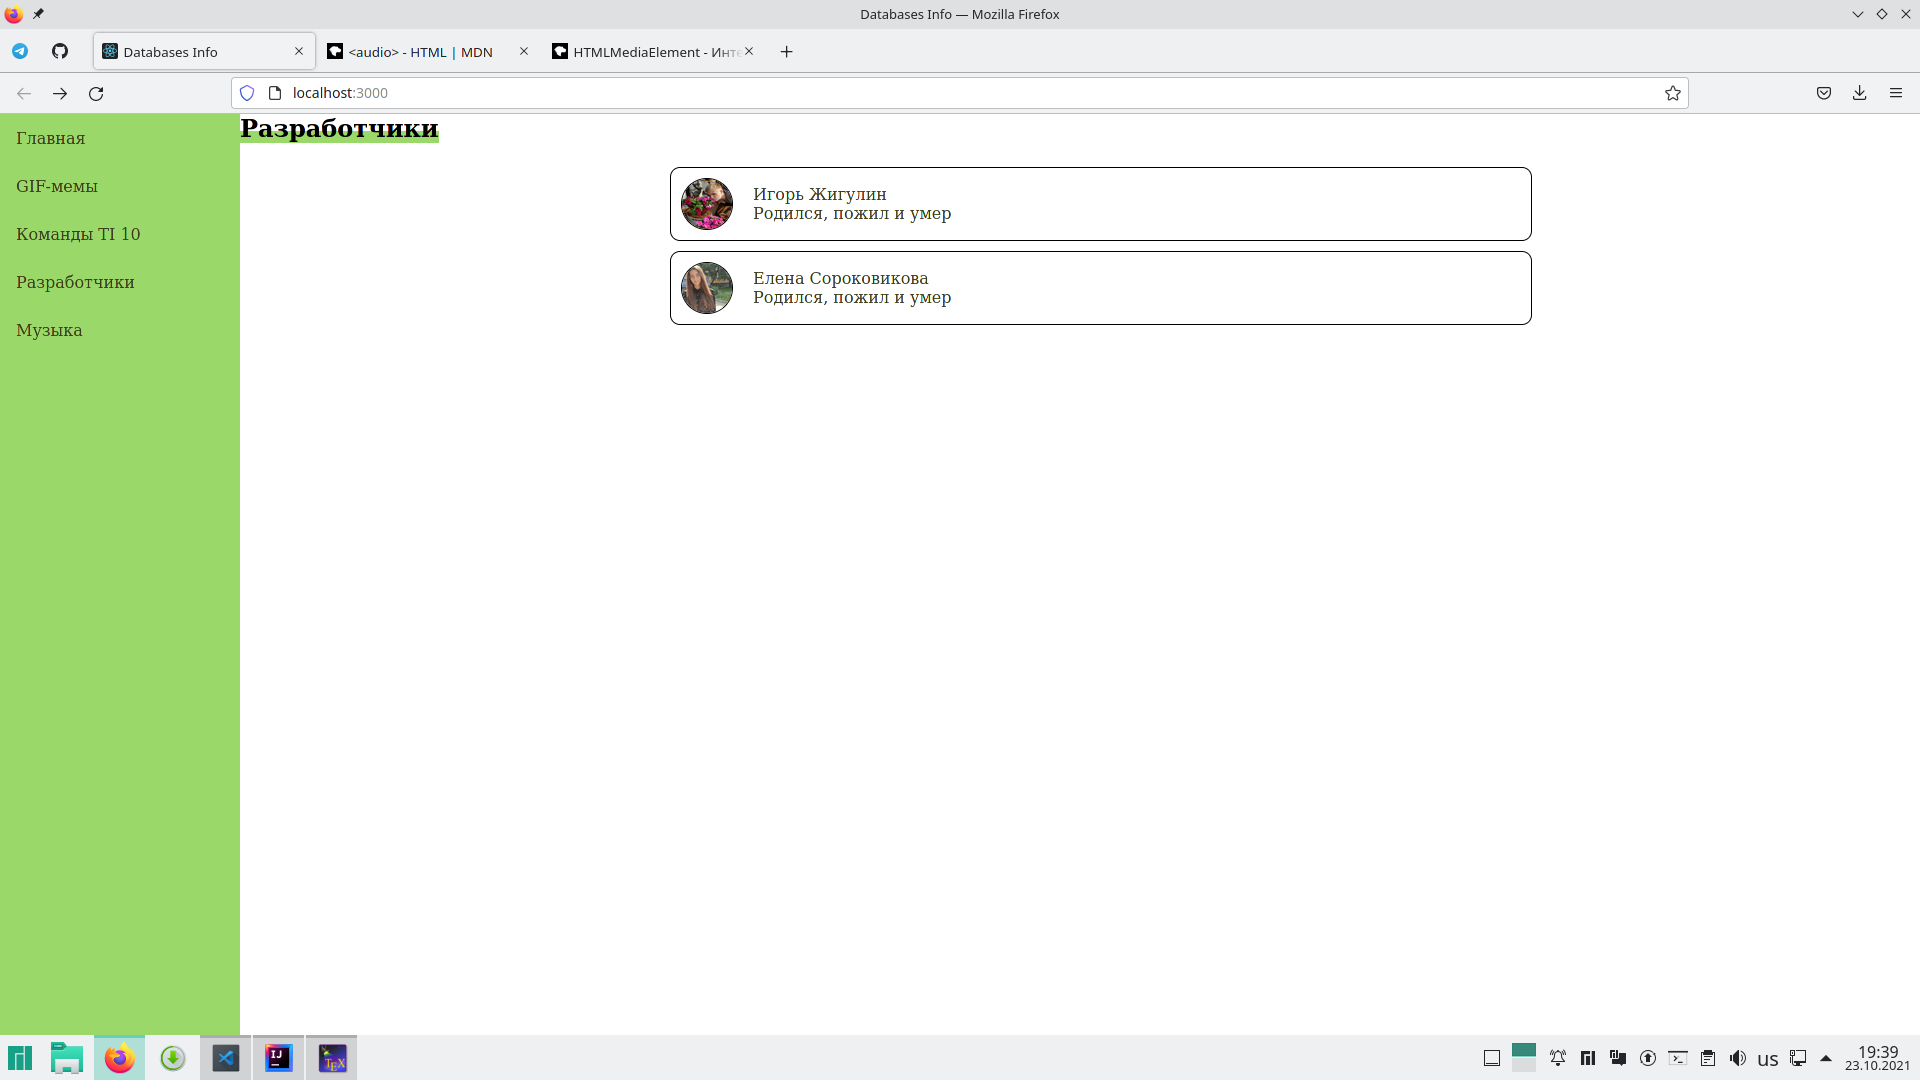
\includegraphics{04}
	\caption{Третья статья специфичной мастер-страницы}
\end{figure}

\section{Вывод}
В ходе выполнения лабораторной работы были изучены принципы работы мастер-страниц в ASP.NET Core MVC. Также были разработаны две мастер-страницы: для всего проекта и для лабораторной работы. Мастер-страницы работают должным образом и позволяют вынести дублирующий функционал в один файл, который будет автоматически подключаться каждый раз при формировании представления.

\end{document}




